\section*{Transformers} \label{sec:Transformers}
These elements consume no power, and convert voltages and currents.
\begin{itemize}[noitemsep, nolistsep]
	\item $\frac{v_{1}}{v_{2}} = \frac{N_{1}}{N_{2}} \longleftarrow$ Voltage Change
	\item $\frac{i_{1}}{i_{2}} = -\frac{N_{2}}{N_{1}} \longleftarrow$ Current Change
\end{itemize}
\vspace{-4.75mm}

	\subsection*{Representations for Turns} \label{subsec:Turn Representations}
		There are 3 common ways to represent the number of turns in a transformer:
		\begin{enumerate}[noitemsep, nolistsep]
			\item $N_{1} : N_{2}$
			\begin{itemize}[noitemsep, nolistsep]
				\item Both $N_{1}$ and $N_{2}$ are integers
			\end{itemize}
			\item $1 : n$
			\begin{itemize}[noitemsep, nolistsep]
				\item The first term might not be $1$, if there isn't perfect division, i.e. $2 : 5$ will not be reduced to $1 : \frac{5}{2}$
				\item $n = \frac{N_{2}}{N_{1}}$
				\item This is the form generally used by our textbook
			\end{itemize}
			\item $a : 1$
			\begin{itemize}[noitemsep, nolistsep]
				\item The second term might not be $1$, if there isn't perfect division, i.e. $2 : 5$ will not be reduced to $\frac{2}{5} : 1$
				\item $a = \frac{N_{1}}{N_{2}}$
				\item This is the form generally used by utility companies
			\end{itemize}
		\end{enumerate}
		\vspace{-5mm}
		
	\subsection*{Reflecting Elements} \label{subsec:Element Reflection}
		There are only 3 equations:
		\begin{enumerate}[noitemsep, nolistsep]
			\item $\frac{v_{1}}{v_{2}} = \frac{N_{1}}{N_{2}} \longleftarrow$ Voltage Change
			\item $\frac{i_{1}}{i_{2}} = -\frac{N_{2}}{N_{1}} \longleftarrow$ Current Change
			\item $Z_{1} = \frac{Z_{2}}{n^{2}}$, as seen in Figure~\ref{fig:Transformer Reflecting}
			\item A negative can be in any one of these, depending on the dot orientation
		\end{enumerate}
		\begin{figure}[ht!]
			\centering
			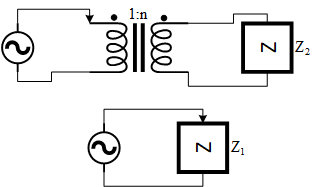
\includegraphics[scale=0.375]{Transformer_Reflecting.png}
			\caption{Transformer Reflecting Elements}
			\label{fig:Transformer Reflecting}
		\end{figure}
		\vspace{-10mm}